%
% $RCSfile: wrapper.tex,v $
%
% Copyright (c) 2004. Christian Heller. All rights reserved.
%
% No copying, altering, distribution or any other actions concerning this
% document, except after explicit permission by the author!
% At some later point in time, this document is planned to be put under
% the GNU FDL license. For now, _everything_ is _restricted_ by the author.
%
% http://www.cybop.net
% - Cybernetics Oriented Programming -
%
% http://www.resmedicinae.org
% - Information in Medicine -
%
% @author Christian Heller <christian.heller@tuxtax.de>
%

\paragraph{Wrapper}
\label{wrapper_heading}

The \emph{Wrapper} pattern \cite{gamma1995} allows otherwise imcompatible
classes to work together. It can be seen as skin object enclosing (wrapping) an
inner core object, to which it provides access. In other words: It adapts the
interface of a class which is why Gamma et al. call the pattern \emph{Adapter}.

\begin{figure}[ht]
    \begin{center}
        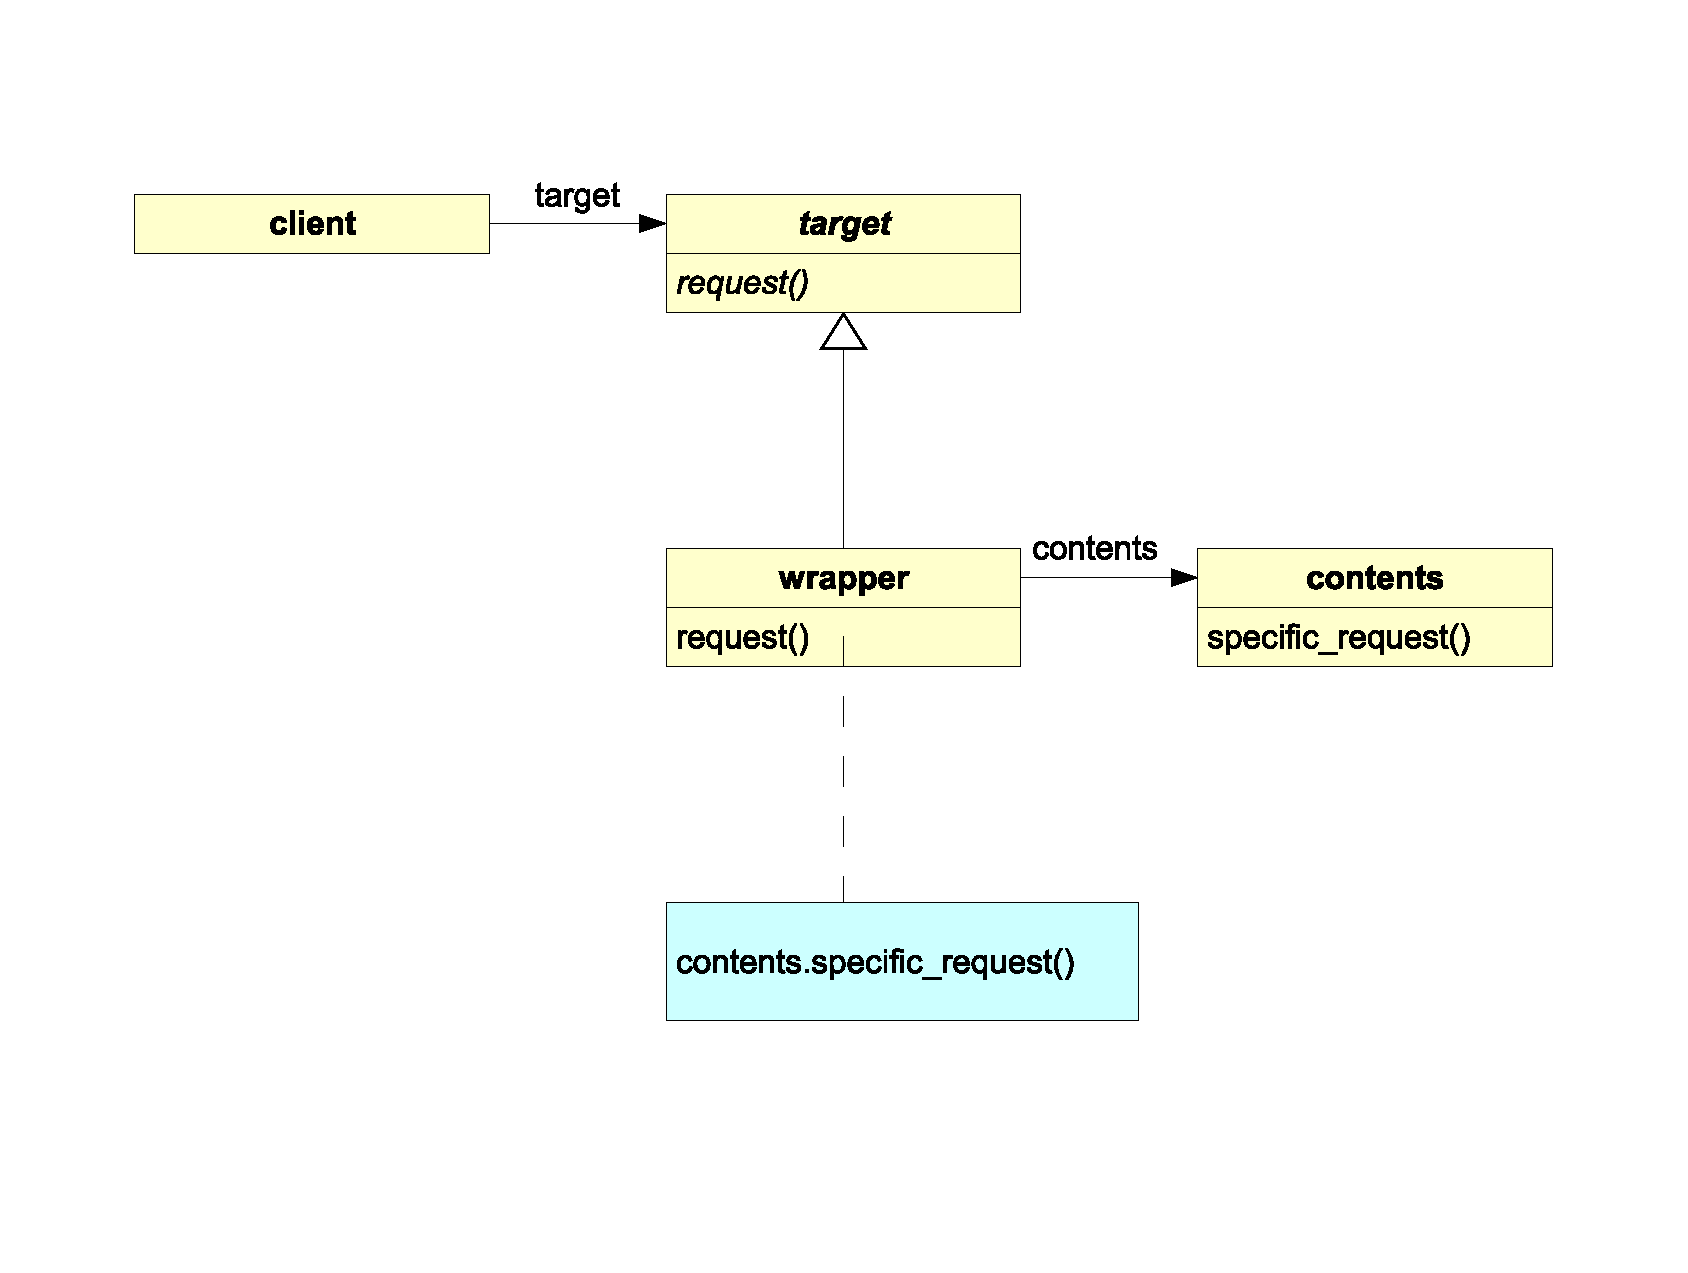
\includegraphics[scale=0.3]{vector/wrapper.eps}
        \caption{Wrapper Pattern}
        \label{wrapper_figure}
    \end{center}
\end{figure}

As can be seen in figure \ref{wrapper_figure}, this pattern makes heavy use of
\emph{Delegation}, where the \emph{Delegator} is the adapter (or wrapper) and
the \emph{Delegate} is the class being adapted \cite{portland}.
